\documentclass[../../main.tex]{subfiles}  % Same level as chapter file, so same path
\graphicspath{{\subfix{../Plots/}}}

\begin{document}

\section{Section structure}

	\subsection{subsection}

	\subsubsection{subsubsection}

\section{Content examples}

	\subsection{Citations}

	Woo! 
	Chapter 2!
	Here's how to cite a random paper\supercite{aartsSolutionDependencyUsing2014}. 
	According to \citeauthor{aartsSolutionDependencyUsing2014} \citeyear{aartsSolutionDependencyUsing2014}, you can also do it this way.
	See bibliography.bib for doing references.

	\subsection{Abbreviations}

	The \verb|glossaries| and \verb|glossaries-extra| packages help you manage the insertion of abbreviations, applied programmatically when inserted with the commands below. 
	Take a look at the \verb|abbreviations.tex| file to see how they're defined.
	Review the documentation for exhaustive command list.

	\begin{verbatim}
		\gls{erp}		 % first instance expanded
		\gls{erp}		 % second + thereafter truncated
		\glspl{erp}		% plural
		\Acrfull{erp}		% force full expansion, capitalize
	\end{verbatim}

	Produces: 
	\begin{enumerate*}[label=(\roman*), itemjoin={{, }}, itemjoin={{, }}, itemjoin*={{, and }}]
	\item \gls{erp}
	\item \gls{erp}
	\item \glspl{erp}
	\item \Acrfull{erp}
	\end{enumerate*}

	\subsubsection{Compositionality}

	The original implementation of this template utilized the \verb|acronym| package, though the \verb|glossaries| package allows more flexibility and control over more complicated cases.
	For example, \verb|glossaries| by default sorts your defined terms alphanumerically before rendering them in your \gls{loa} page. 
	This is more ideal for compositionality in your abbreviations (i.e. using small acronyms as building blocks for others). 
	See the code in \verb|abbreviations.tex| that generates the following example case and their appearance in the \gls{loa}: 
	\begin{displayquote}  % uses the csquotes package
		``\gls{nmda} elicits responses from \glspl{nmdar}. 
		A variety of neuropsychiatric disease states are associated with \gls{nrh}.''	
	\end{displayquote}

	\subsubsection{Alternate forms}

	One more noteworthy feature of \verb|glossaries| I'll draw your attention to is the ability to define alternate versions of your acronyms for terms used interchangeably.
	This is done using wrapper commands that check for user-defined inputs in definitions.
	For example, in neuroscience: 
	
	\begin{displayquote}
		``\glspl{ap} emitted by a brain cell are often referred to as \altglspl{ap}.''
	\end{displayquote}

	Both of these commands will link back to the defintion of \glspl{ap} in the \gls{loa}.
	This is one of a variety of ways you could possibly implement and customize your management of abbreviations.

	\subsection{SI units}

	The \verb|siunitx| package allows us to insert units in a typographically consistent way, ensuring proper height, spacing, and proper formatting of units (e.g. prevention of linebreaks).
	It's desirable in this context for much the same reasons as the \verb|acronym| package.

	% millimolar is not an SI unit, but we can define it ourselves
	% defined in usercommands.tex as
	% \DeclareSIUnit{\mM}{mM}        % millimolar


	\begin{displayquote}
		``The concentration of drug was \SI[per-mode=fraction]{0.02}{\mol/\L} (\SI{20}{\mM}), which can also be formatted as \SI[per-mode=fraction]{0.02}{\mol\per\L}.
		After a \SI{30}{\minute} period for pharmacological action, mice were placed in a chamber, anesthetized under \qty{3}{\percent} isoflurane, then fixed in a nose cone delivering the same anesthetic mixture. 
		Samples were extracted, tin foil wrapped, and placed in a \SI{-80}{\degreeCelsius} freezer for 25 minutes to achieve firmness.''
	\end{displayquote}

	\subsection{Equations}

	Here I'll show you how to use some math, incorporating some more examples of units and abbreviations.

	\Acrfull{csd}, $\Phi$, was calculated by a numerical approximation of the second spatial derivative of voltage, expressed as:

	\begin{equation}
		\Phi_{t, c} = -\frac{\phi_{t, c+1} - 2\phi_{t, c} + \phi_{t, c-1}}{\Delta c^2 \times g}
	\end{equation}

	where $\phi_{t, c}$ represents recorded voltages at time-point $t$ and channel $c$ on the linear electrode array, such that constant $\Delta c$ is the spacing between adjacent contacts. 
	The constant $g$ represents the conductivity of the extracellular medium, defined for these analyses as \SI[per-mode=fraction]{0.3}{\siemens/\m}, consistent with putative bounds of extracellular impedance measurements (\qtyrange[range-units=single,range-phrase=-]{\sim 0.3}{0.6}{\siemens\per\m}) for frequencies below \SI{10}{\kHz}. 
	% notice how \siemens\per\m, when attached to a constant, is a fraction, but uses exponent notation when expressed for a range
	Checkout the code that generates these units. 

	\subsection{Figures}

	\begin{figure*}[hb] % place approximately here 'h', OR at the bottom 'b' of the page (adding 'b' relaxes the demand)
		\centering
		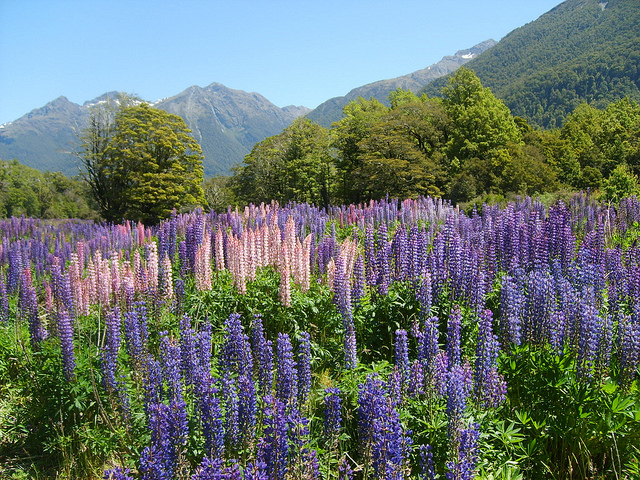
\includegraphics[height =4in]{./Plots/nature.jpg} 
		\caption{An individual figure!}
	\end{figure*}
			
	\begin{figure}[H] % place float exactly here 'H'
		\subfloat[\label{fig:HD8538_ellplot}]{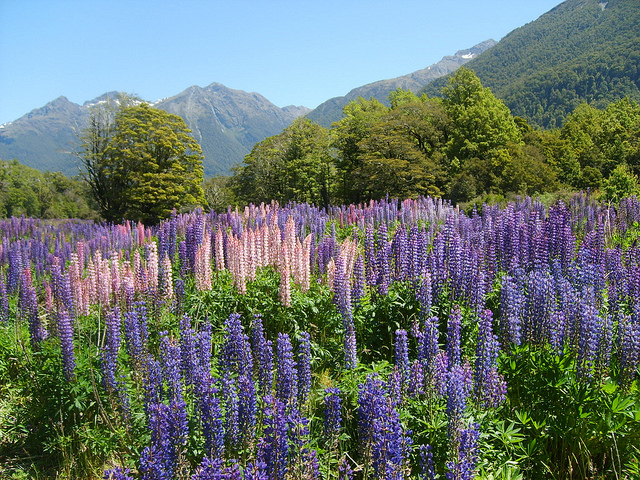
\includegraphics[height =2.5in]{./Plots/nature.jpg}} 
		\subfloat[\label{fig:HD8538_phot}]{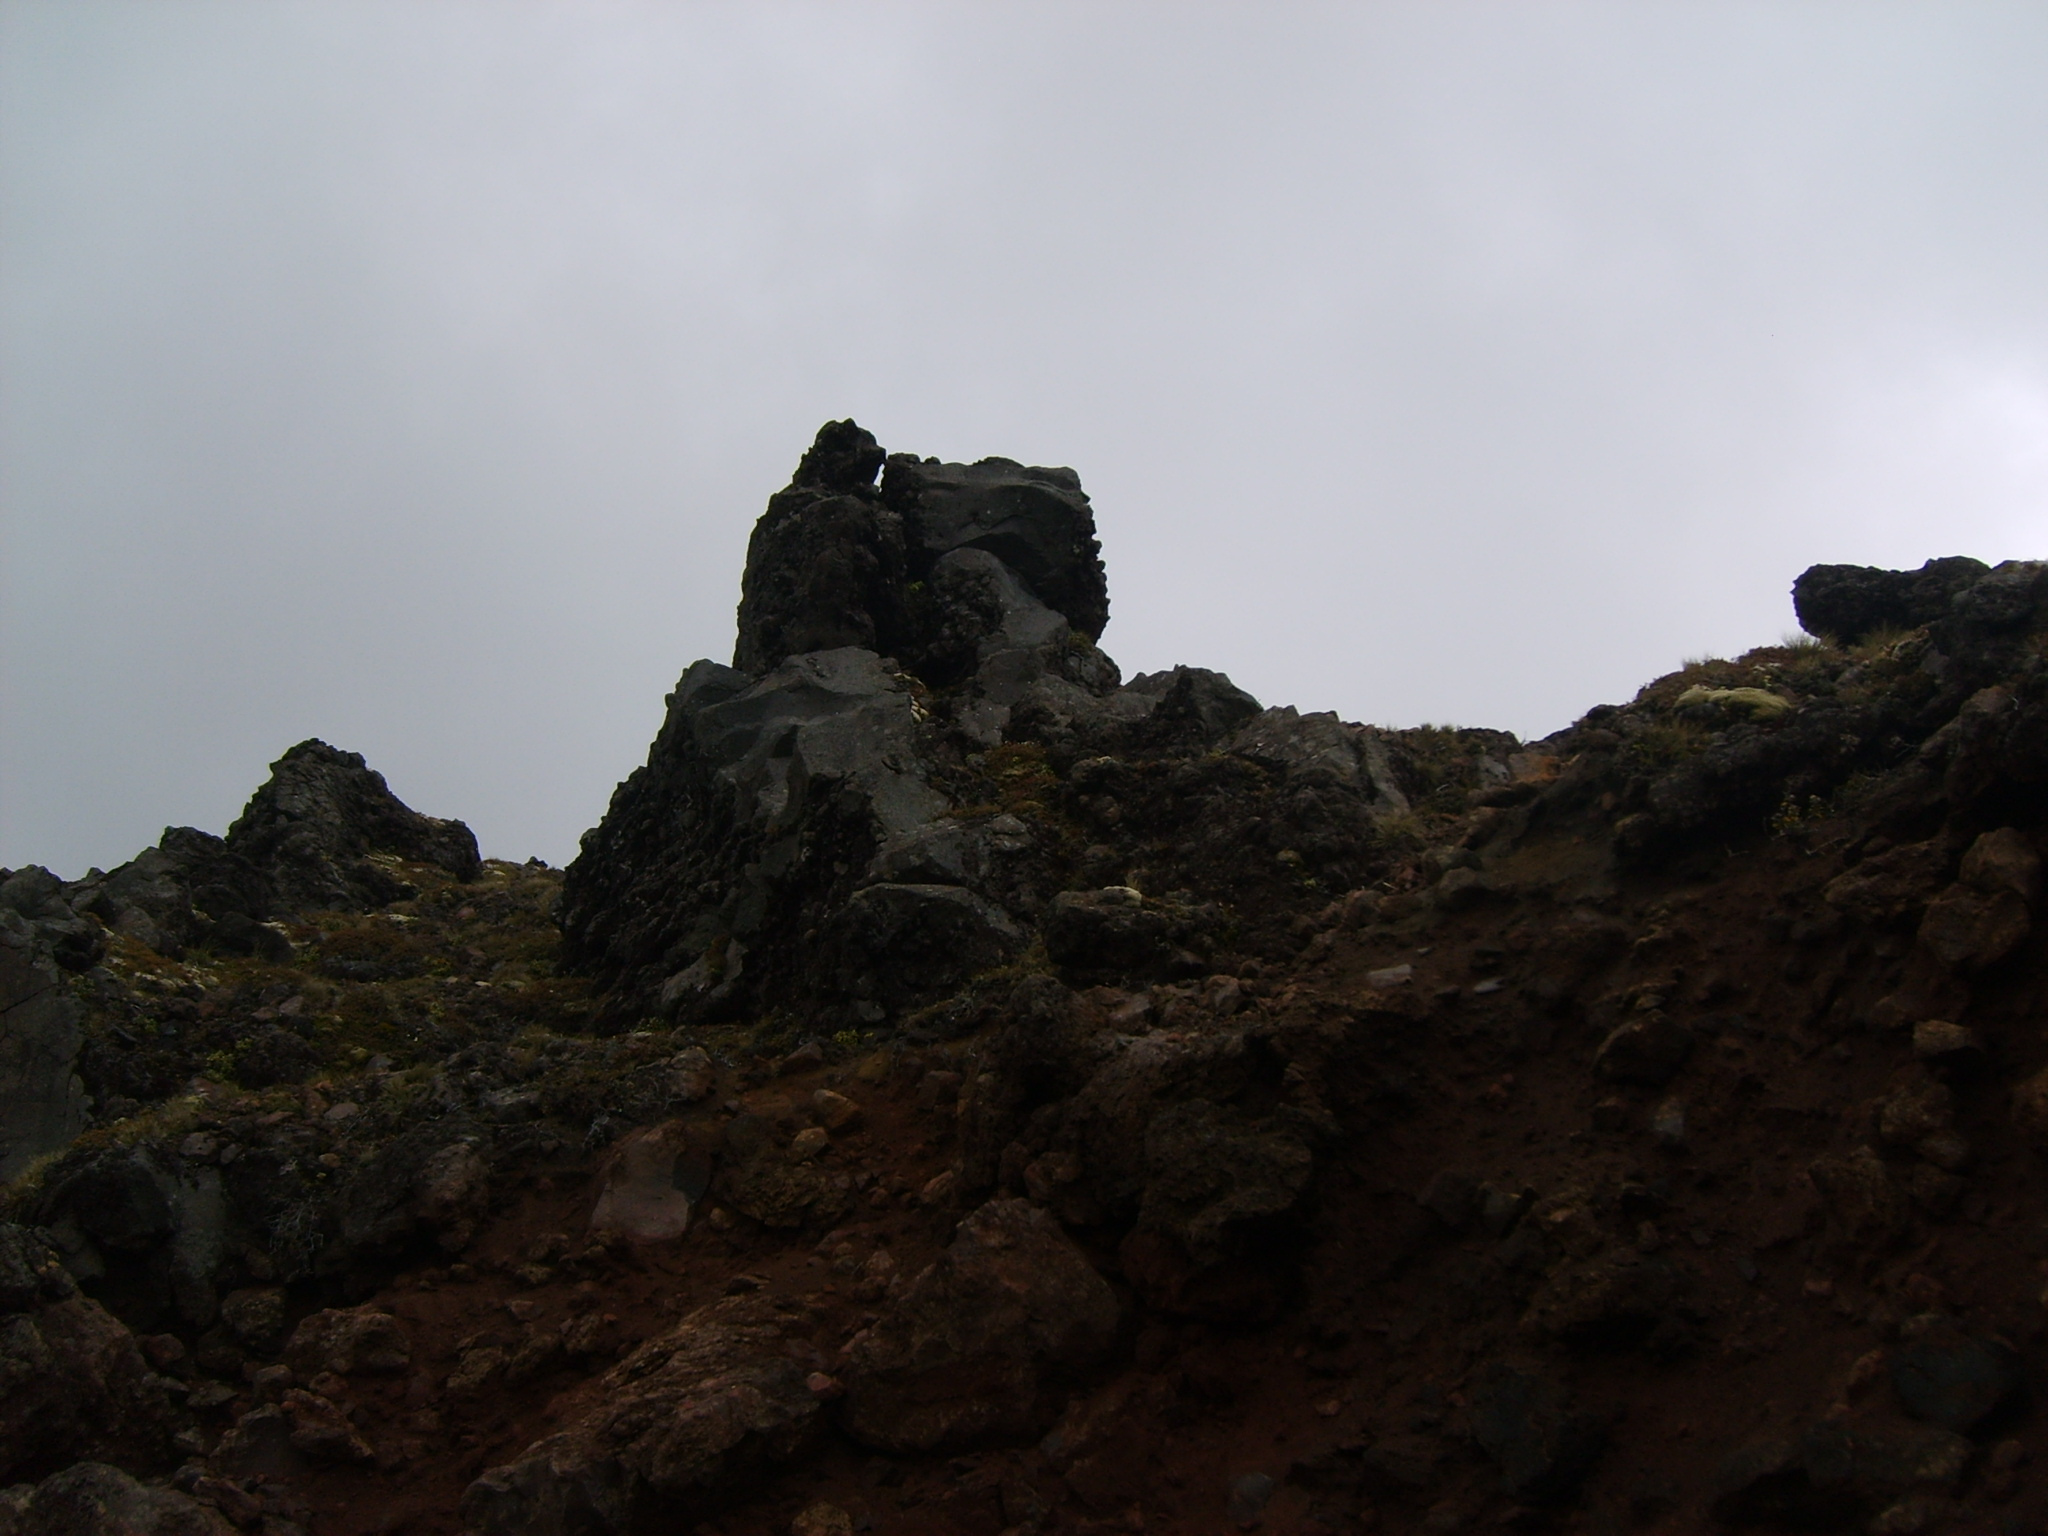
\includegraphics[height =2.5in]{./Plots/rocks.jpg}} \\
		\subfloat[\label{fig:HD8538_vis}]{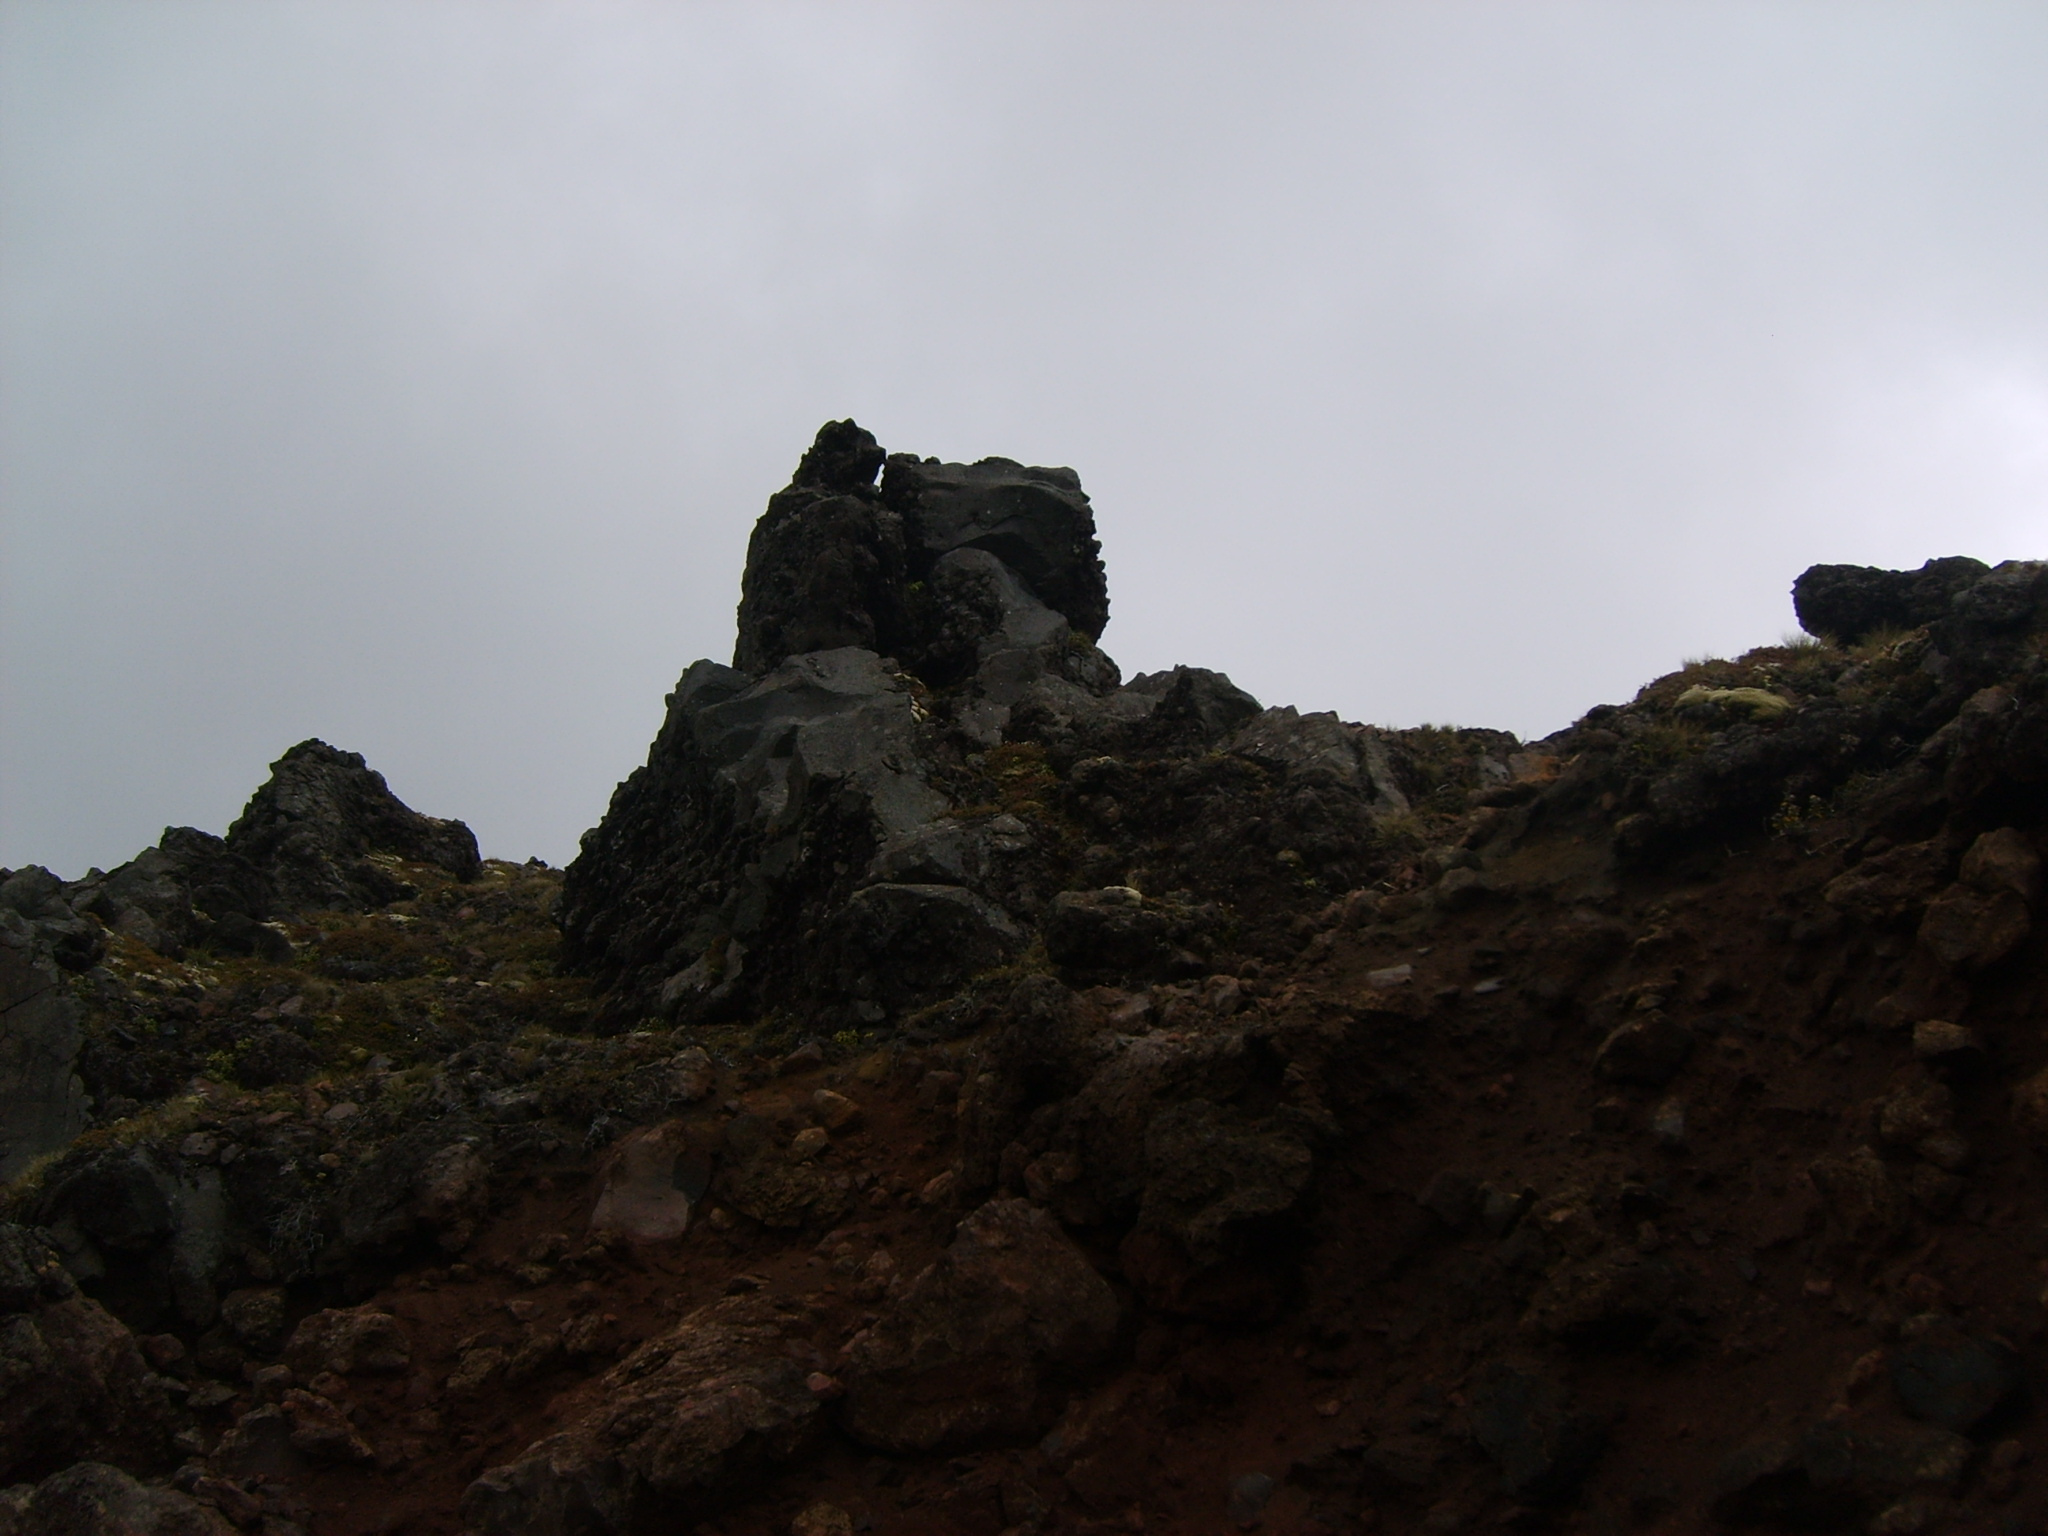
\includegraphics[height =2.5in]{./Plots/rocks.jpg}}
		\subfloat[\label{fig:HD8538_HRD}]{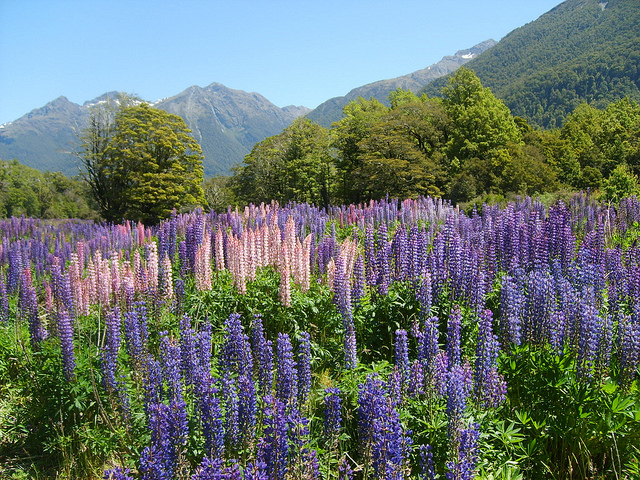
\includegraphics[height =2.5in]{./Plots/nature.jpg}}
		\caption{Multiple figures!}
	\end{figure}


	\subsection{Tables}
	\begin{landscape}
\begin{longtable}{cccccccccccccc}
\label{tab:disk}\\
\caption{Insert Table Caption here}\\
\hline\endhead  % header material
\hline\endfoot  % footer material
\hline
Blah & Blah & Blah \\
\hline
Stuff & Things & etc. \\
\nodata & \nodata & \nodata \\
\end{longtable}
\end{landscape}


\end{document}